% =========================================================
\section{Motivation -- Why regularize ?}

\begin{frame}{From ERM to Regularization}
	\textbf{Empirical Risk Minimization (ERM)} chooses parameters that fit best the training dataset $S$.
	\[
	\hat{\bbeta}_{\text{ERM}} \,\in\, 
	\arg\min_{\bbeta}\;
	\underbrace{
	\frac{1}{n}\sum_{i=1}^n \ell\left(y_i \,,\, f_{\bbeta}(x_i)\right)
	}_{L_S(f_{\bbeta})}
	\]
	\begin{itemize}
		\item If the model is flexible, ERM can fit noise $\Rightarrow$ \textbf{overfitting}.
		\item We want good performance on \textbf{unseen data}: minimize \textbf{test/true risk} $L_D(f_{\bbeta})$.
		\item Key idea: control model complexity to reduce the \textbf{generalization gap}.
	\end{itemize}
\end{frame}

\begin{frame}{Regularization as a complexity control knob}
	\textbf{Regularized objective:}
	\[
	\hat{\bbeta} \,\in\, \arg\min_{\bbeta}
	\left[\;
	\underbrace{L_S(f_{\bbeta})}_{\text{Loss}}
	\;+\; {\color{red}\lambda} \times \underbrace{\Omega(f_{\bbeta})}_{\text{Penalty}}
	\;\right]
	\]
	\begin{itemize}
		\item $L_S(f_{\bbeta})$ : Empirical error over $S$ (MSE, 0-1 loss, \dots)
		\item $\Omega(f_{\bbeta})$ : complexity penalty (norm/quasi-norm)
		\item ${\color{red}\lambda}>0$ : trade-off parameter
	\end{itemize}
\end{frame}

\begin{frame}{Why overfitting happens (bias variance trade-off)}
	\begin{itemize}
		\item Increasing model complexity typically:
		\begin{itemize}
			\item \textbf{decreases bias} (model can fit more patterns),
			\item \textbf{increases variance} (model becomes sensitive to noise/data changes).
		\end{itemize}
	\end{itemize}
	A classic view of expected test error (conceptually):
	\[
	\color{red}
	\mathbb{E}\big[L_D(h \in \mathcal{H})\big] \;\approx\; \text{Bias}^2 + \text{Variance} + \text{Noise}
	\]
	\begin{itemize}
		\item Regularization reduces variance by shrinking / simplifying the solution.
	\end{itemize}
\end{frame}

\begin{frame}{}
	\centering
	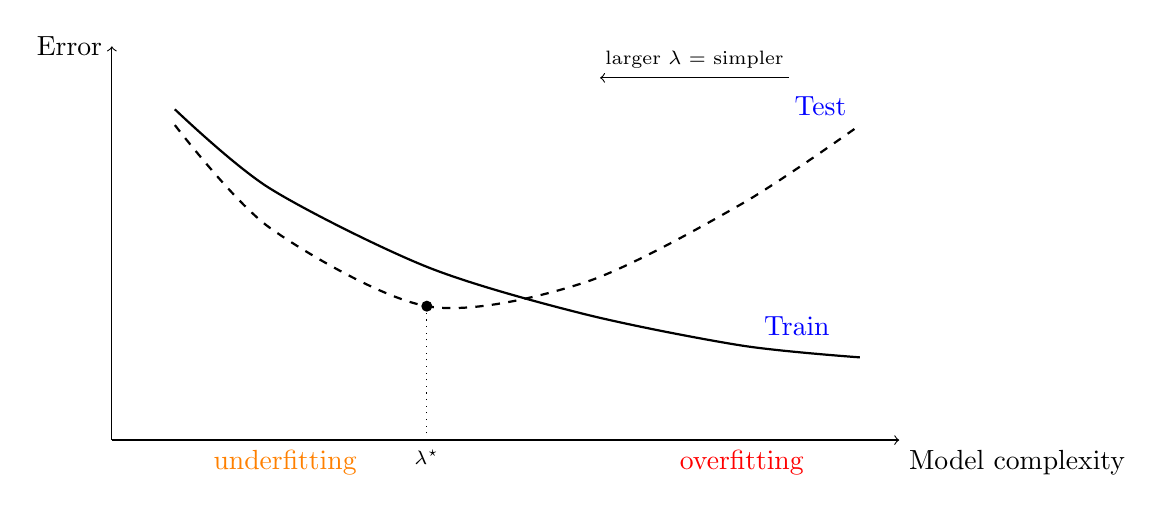
\begin{tikzpicture}[x=1cm,y=1cm]
		% Axes
		\draw[->] (0,0) -- (10,0) node[below right] {Model complexity};
		\draw[->] (0,0) -- (0,5) node[left] {Error};
		
		% Regions labels
		\node[below] at (2.2,0) { \textcolor{orange}{underfitting}};
		\node[below] at (8.0,0) { \textcolor{red}{overfitting}};
		
		% Train curve (decreasing)
		\draw[thick] plot[smooth] coordinates {(0.8,4.2) (2,3.2) (4,2.2) (6,1.6) (8,1.2) (9.5,1.05)};
		\node[above] at (8.7,1.2) {\textcolor{blue}{Train}};
		
		% Test curve (U-shape)
		\draw[thick,dashed] plot[smooth] coordinates {(0.8,4.0) (2,2.7) (4,1.7) (6,2.0) (8,3.0) (9.5,4.0)};
		\node[above] at (9.0,4.0) {\textcolor{blue}{Test}};
		
		% Best point
		\fill (4,1.7) circle (2pt);
		\draw[dotted] (4,0) -- (4,1.7);
		\node[below] at (4,0) {\scriptsize $\lambda^\star$};
		
		% Lambda arrow
		\draw[->] (8.6,4.6) -- (6.2,4.6);
		\node[above] at (7.4,4.6) {\scriptsize larger $\lambda$ = simpler};
	\end{tikzpicture}
	
	\vspace{0.6em}
	\small Regularization controls complexity $\Rightarrow$ better generalization.
\end{frame}

% =========================================================
\section{Objective -- Why we aim for sparse models ?}

\begin{frame}{What is sparsity?}
	\textbf{Definition :} A model is \textbf{sparse} if many parameters are \textbf{exactly zero}.
	\begin{itemize}
		\item Linear models: $y \approx X\bbeta$
		\item Define the \textbf{support} (selected features):
		\[ 
		{\color{red}
		\mathrm{supp}(\bbeta)=\{\,j\,:\,\beta_j\neq 0\,\}} \quad,\quad 
		{\color{red}
		|\mathrm{supp}(\bbeta)| = \norm{\bbeta}_0}
		\]
		\item Sparsity means: only a small subset of features truly “matters”.
	\end{itemize}
\end{frame}

\begin{frame}{Why sparse models are preferred ?}
	\begin{itemize}
		\item \textbf{Interpretability:} easier to explain which variables drive predictions.
		\item \textbf{Measurement / data cost:} fewer features to collect (medical, finance, IoT, \dots).
		\item \textbf{Robustness:} reduces reliance on noisy/irrelevant variables.
	\end{itemize}
\end{frame}


\begin{frame}{Sparsity illustration}
	\centering
	\begin{tikzpicture}[>=Latex]
		\node[draw, rounded corners, inner sep=6pt] (v) {$\bbeta = \begin{bmatrix}
				2.3\\ 0\\ 0\\ -1.1\\ 0\\ 0\\ 0.7\\ 0
			\end{bmatrix}$};
		
		\node[below=0.9cm of v, align=center] (t) {\textbf{Sparse:} only 3 non-zeros\\
			Selected features: $\mathrm{supp}(\bbeta)=\{1,4,7\}$};
		\draw[->] (v) -- (t);
	\end{tikzpicture}
\end{frame}
